\chapter{并行树状概率模型}
在本章中,我们将这个目标词表示扩展到一个分层的形式,使它们适配基于树的分层概率计算。首先,我们提出了一个在分层结构上建模参数的字编码方案。因此,考虑到GPU上的并行吞吐性能,我们推导出紧凑的代价函数及其梯度。同时,树上的单词分布对其性能有很大的影响,应该在训练阶段之前定义,这些动态交换算法在训练过程中改变了单词群或子树结构在这个研究中。我们采用了几个分层聚类和词汇分割策略,用统计,句法和语义知识来初始化其结构,以达到一个稳定和可以预期的性能。而且,在推理过程中,不同于传统的softmax情况,得到最好的候选者自然是可行的,层次推理不能直接用 softmax 方法来实现。我们讨论基于树的搜索策略的两种不同的推理情况:a)打分:输出给定序列的概率;b)排序   :在给定的上下文中获取得分最高的一个候选单词。
\section{基于二叉树的单词极性编码}
首先,所有的单词分布在二叉树的叶节点上,因此我们可以通过访问从根到叶节点的所有内部节点来定位每个特定的词,所以不同的访问路径代表不同的单词。在这里,单词$ w $的路径表示所有内部节点$ \theta^w_i $和它访问的边$ d ^ w_i $。

我们接下来详细说明模型的编码方式。其中,$ \theta_i ^ w $表示到达单词$w$的路径上的$ i^{th} $层上的非叶节点,并且$\theta_i ^ w$是一个 $m$维度的向量,$ \theta_i ^ w \in\mathbb{R}^m $ 其中$ i \in [0, l ^ w - 1] $。同样的,$ d_i ^ w $表示连接第$(i-1)^ {th} $和$ i ^ {th} $层节点的边。对于每个非叶子节点来说,向下移动到左边的分支标记为$ -1 $,选择正确的分支标记为$ + 1 $。因此,在$i\in[0,l^w-1]$, $d_i^w\in \{-1,+1\}$。 此外, $l^w$~表示从根到叶单词的路径长度。如果该二叉树是平衡树,即单词都均匀分布在同一层叶子节点上,那么树深是$l^w\approx \log \mathcal{|V|}$ 。通过这个方案,我们可以通过表示极性路径来定位每个单词,将单词索引(Indexing)或二元稀疏表示(One-hot Representation)改变为单词极性编码元组$(d ^ w,\theta ^ w)$。


在用python语言实现过程中,我们通过维护一个路径查找表$\Gamma$(Lookup Table),记住每个单词$ w $从根到叶的所有访问内部节点的索引。这样,通过从$ \Gamma(w)$中选择对应行的所有节点,从参数矩阵${\Theta} $中检索$ \theta ^ w $。其中${\Theta} $的第一维的维度是:
\begin{equation}\label{equ:sums}
\sum_{i=0}^{\log \mathcal{|V|}}{2^i} = \mathcal{|V|} -1.
\end{equation}
因此,p-tHSM模型没有增加模型额外参数,除了预先给定的路径查找表$ \Gamma $。

除此以外,我们通过从矩阵$\mathcal{D}$中获得$w^{th} $行向量来检索$d^w$,其中$w$是词汇表中的单词索引。 此外,$\{\Gamma,\mathcal{D}\}$ 是由层次聚类算法预先给定的,$\Theta$是通过训练数据集上的代价函数的梯度下降来优化的。为了保证理解正确,我们在这里再一次强调$ \Theta $是模型的参数,$ \Gamma $记忆路径节点索引信息,$\mathcal {D}$取 $ \{ - 1,+1 \} $中的值。

如图~\ref{fig:tree_hsm}~所示,内部参数向量 $\theta_i^w$, 边 $d_i^w$ 并且单词在树的叶子节点上。除此之外, 加粗的那条路径从根节点到叶子节点 $w$ 被定义为参数对 $(d^w,\theta^w)$。其中 $d^w$ 是一个向量, $\theta^w$ 是一个参数矩阵. 例如, 图里面的参数实际结果是 $d^w=[-1,+1,-1]$ , $d^{v}=[-1,+1,+1]$。
\begin{figure}[!h]
  \centering
    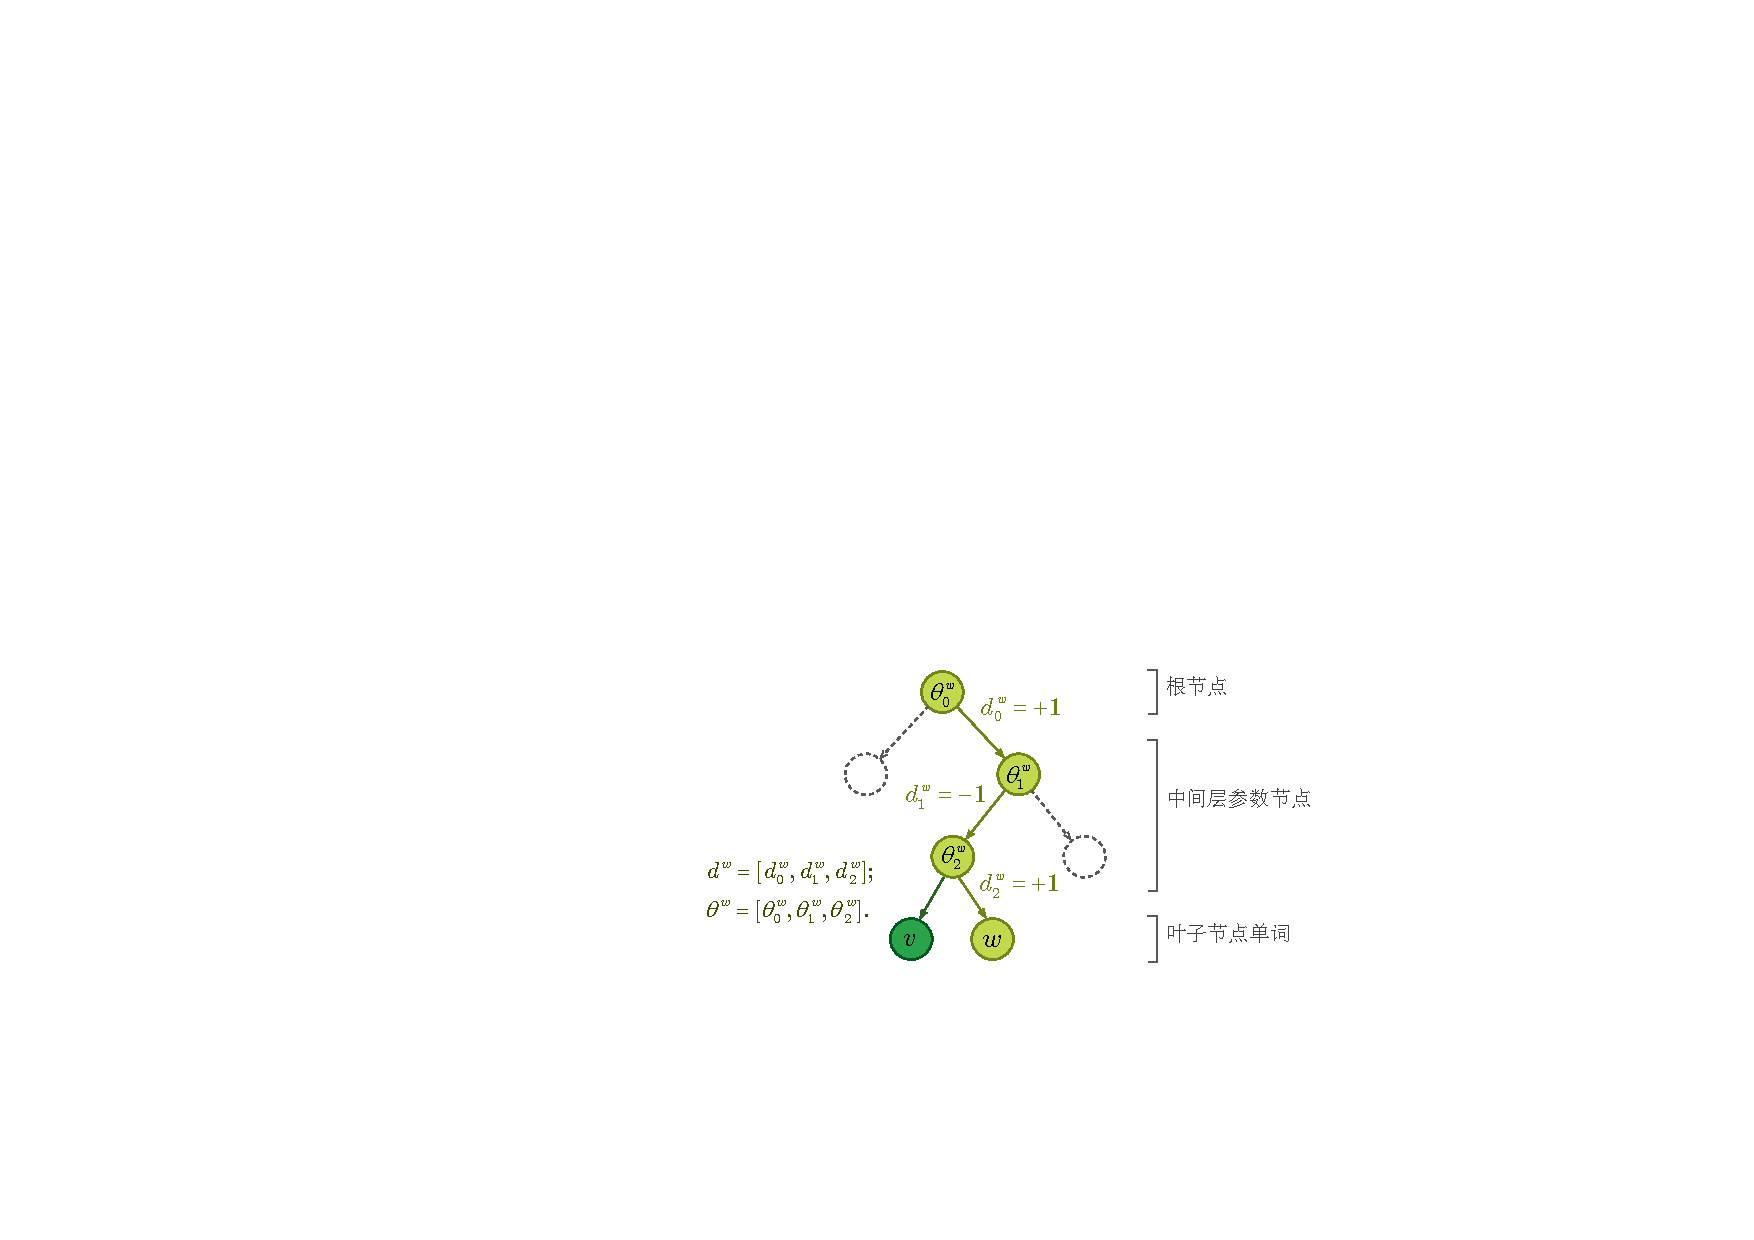
\includegraphics[width=0.9\linewidth]{./figures/thsm.pdf}
\caption{树状层次概率模型}\label{fig:tree_hsm} %
\end{figure}

\section{基于二叉树的代价函数和导数}
在目标词树的每个步骤中,我们对每个非叶节点是左下分支还是右分支进行逻辑预测。 给定$ i^{th} $节点和隐藏层$ h $的$ i^{th} $ 标签 $d^w_i\in \{-1,1\}$的概率为:
 \begin{equation}
p(d^w_i|\theta_{i}^w,h) =\sigma(\theta_{i}^w h)^{d_i^w}\times(1-\sigma(\theta_{i}^w h))^{1-{d_i^w}},d_i^w \in [0,1]
\end{equation}
其中$ \sigma(z)= 1 /(1 + \exp(-z))$表示 $\sigma$ 函数。根据 $\sigma$ 函数的对称性规则:$\sigma(z)+ \sigma(-z)=1 $,可以用来帮我们把公式缩写成:
 \begin{equation}
p(d^w_i|\theta_{i}^w,h) =\sigma(\theta_{i}^w h)^{d_i^w}, d_i^w \in [-1,1]
\end{equation}
更进一步,我们可以将公式缩写成以下形式:
\begin{equation}
p(d^w_i=\pm 1|\theta_{i}^w,h) = \sigma({d_i^w}\theta_{i}^w h)
\end{equation}



 因此,单词$ w $的概率是从根到相应叶节点的路由概率$(d^w,\theta^w)$的联合乘积:
\begin{equation}\label{equ:pw}
\begin{split}
 \log p(w|h)=&\log\prod_{i=0}^{l^w-1} p(d^w_i|\theta_{i}^w,h) = \sum_{i=0}^{l^w -1} \log\sigma(d_i^w \theta_{i}^w h)\\
 =&\log\sigma({d^w}^\top \theta^w h)=\zeta(- {d^w}^\top \theta^w h )
 \end{split}
\end{equation}
其中 $\zeta(z)$ 代表 softplus 函数: $\zeta(z)= \log (1+\exp(z))$。 该函数的导数是 $\sigma$ 函数, 其导数计算公式是: ${\mathrm{d}\zeta(z)}/{\mathrm{d} z}= \sigma(z)$~\upcite{DBLP:conf/nips/DugasBBNG00}。如图所示, softplus 函数通常被视为 ReLU函数的替代函数,因为他们两个函数除了零点附近分布不一样以外,其他地方分布相同。但是softplus函数在零点附近可导,ReLU函数在零点附近不可导。
\begin{figure}[!ht]
  \centering
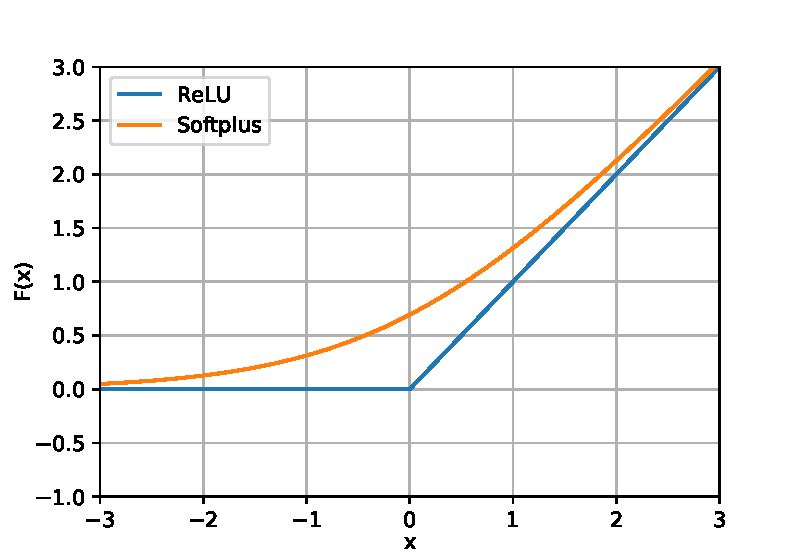
\includegraphics[width=0.6\linewidth]{./figures/relus.pdf}
\caption{Softplus和ReLU函数的示意图}\label{fig:soft}
\end{figure}

接下来,我们给出模型相应的损失函数$ \ell(\theta | h,w)$,它是定义在二叉树上面的负对数似然函数(Negative Log-Likelihood,NLL):
\begin{equation}\label{equ:cost}
\begin{split}
   \ell(\theta|h,w) =&-\log\prod_{i=0}^{l^w -1} \sigma(d_i^w \theta_{i}^w h) = -\log \sigma({d^w}^\top \theta^w h)\\
    =& \log (1+\exp(- {d^w}^\top \theta^w h )) =  \zeta(- {d^w}^\top \theta^w h )
\end{split}
\end{equation}
从此公式中,我们可以发现最小化基于树的负对数似然值,意味着直接最大化softplus损失和估计字的概率。

尽管如此,在传统的tHSM算法中,该模型逐层计算每个节点的对数概率。 因此,这个词的整体联合对数概率通过各层线性相加。 因此tHSM的时间复杂度为$\mathcal{O(|H|\log|V|})$,其计算公式为:
\begin{equation}
\ell(\theta|h,w) =\sum_{i=0}^{l^w-1} \{(1-d'^w_i)\log (\sigma(\theta_{i}^w h))  + {d'^w_i}\log (1-\sigma (\theta_{i}^w h))\}
\end{equation}
其中 $d'^w_i\in \{0,1\}$,这两个部分从底到顶,分别对内部节点的左右子树的联合概率进行建模。

值得注意的是,p-tHSM和tHSM算法之间的主要区别在于:a)tHSM算法涉及许多微小的矩阵乘法操作,而在p-tHSM中我们直接将所有参数$(d^w,\theta^w)$ 2D矩阵是以运行时内存消耗为代价的,我们考虑这个向量和相对较大的矩阵的乘法,如图~\ref{fig:tree_hsm}~所示。 b)扣除模型的紧凑损失函数,并行的计算这条路径上所有节点的对数概率而不是逐层计算,为p-tHSM模型提供更好的时间效率。

接下来,模型的所有参数$\{\theta^w,h\}$针对模型的代价函数的导数是 :
\begin{equation}
\begin{split}
\frac{\partial \ell}{\partial \theta^w}=&(\sigma({d^w}^\top\theta^w h) -1){d^w}^\top h \\
\frac{\partial \ell}{\partial h}=&(\sigma({d^w}^\top \theta^w h) -1){d^w}^\top \theta
\end{split}
\end{equation}


二叉树分解的一个主要优点是它避免了在整个词汇表中概率的归一化,因为树中词的汇总概率自然等于1。
\begin{equation}
\sum_{w\in \mathcal{V}}{p(w|h)}=\sum_{w \in \mathcal{V}}\sum_{i=0}^{l^w-1}{\sigma(d_i^w\theta_{i}^w h)}=1.
\end{equation}





\section{基于二叉树的推理算法}
考虑到本章开始提出的第一个问题,即给定序列$ [w_1,\cdots,w_T] $,求该序列的概率。 直观地说,当给定相应的上下文$ h $时,我们可以通过获取一个特定单词$ w $的概率或对数概率来分解问题:
\begin{equation}
\begin{split}
    p(w|h) =&\sigma({d^w}^\top \theta^w h)\\
   \log p(w|h) =& -\zeta(- {d^{w}}^\top \theta^{w} h )
\end{split}
\end{equation}
其中概率$ p(w | h)$和单词$ w $的对数概率$ \log p(w | h)$可以直接通过等式~\ref{equ:pw}~和~\ref{equ:cost}~逐步计算出来。 因此,我们可以推导出这个序列的概率为:
\begin{equation}
   \log p(w_1,\cdots, w_T)=\sum_{t=1}^T\log p(w_t|h_t) = -\zeta(- {d^{w_t}}^\top \theta^{w_t} h_t )
\end{equation}
显然,这种类型的操作比传统的softmax方法有效得多,它只需要$\mathcal{O}(\mathcal {| H | \log| V |})$计算复杂度,而传统的softmax算法却需要$\mathcal{O}(\mathcal {| H || V |})$。

关于第二种情况(也被称为$\arg\max $方法),即当给定前一个上下文时,在整个词汇表中搜索最有可能的下一个单词(概率最大的单词)。我们可以在选择最上面的一个候选人之前计算词汇表中所有单词的概率。这个过程仍然是昂贵而缓慢的,因为它涉及到整个词的分层树。如在算法~\ref{alog:argmax}中所描述的,为了避免两个小概率的精确度损失问题,计算每个内部节点的对数概率。

而不是搜索全局最优结果,我们可以用局部贪婪算法搜索次优结果。具体而言,对于$ i $ -th层中的节点,当$ p(d ^ w_i | \theta_{i} ^ w,h)\ge 0.5 $时选择左边的分支,相反适用,如算法~\ref{alog:greed_argmax}所示。因此,计算时间复杂度仍然是$ \mathcal{O}(| H | \log \mathcal {| V |})$。


\begin{algorithm}[!ht]
\SetAlgoLined
\KwData{隐藏层输出 $h$;}
\KwResult{ 预测的单词 $w$. }
 路径列表 $\mathtt{path}$=[] \;
\While(\tcp*[h]{逐层搜索}){$k \le \log \mathcal{V}$ }{
\eIf{$p(d_{k} |\theta_{k},h) \ge 0.5$ }{
 $k=  k*2$ \tcp*[r]{左分支}
}{
 $k = k*2+1$ \tcp*[r]{右分支}
}
 $\mathtt{path}$.append($k$) \tcp*[r]{将 $k$ 添加到路径列表}
}
{通过查找$\Gamma$路径表,找出对应的单词}\;
 alter $\mathtt{path}$ with word $w$ by looking-up table $\Gamma$\;
 \Return $w$ \;
\caption{逐层贪心搜索 Argmax}\label{alog:greed_argmax}
\end{algorithm}

\section{基于二叉树的聚类算法}
词汇表中每个单词$(d^w,\theta^w)$的极性编码与树的结构密切相关。对于提出的p-tHSM方法,我们采用了几种树聚类算法来提高其性能和稳定性。这些聚类算法为每个单词生成二进制前缀字符串,表示树中单词的位置,并将用于初始化p-tHSM方法。


1)Unigram 聚类。它根据词频对词汇进行排序,并根据单词统计从底端到顶端进行合并,也称为霍夫曼编码~\upcite{DBLP:conf/nips/MikolovSCCD13}。

2)Bigram 聚类\footnote{布朗聚类:https://github.com/percyliang/brown-cluster}。它是一个层次聚类算法,使用bigram上下文来确定单词的分布相似性,将相似的单词放置在二叉树的附近位置~\upcite{DBLP:journals/coling/BrownPdLM92,liang2005semi}。在将簇大小指定为1之后,它从底部到顶部合并具有一个节点的单词。生成的单词二进制路由正是分层二进制结构的分布。

3)语义聚类\footnote{https://code.google.com/archive/p/word2vec/}。在引导式的方式下,词嵌入在外部语料库上训练,我们将传统的凝聚式聚类应用于字嵌入特征~\upcite{DBLP:books/sp/mining12}。


\section{本章小结}

\chapter{并行层次概率计算模型}
在本章中,我们将这个目标词表示扩展到一个分层的形式,使它们适配基于类和基于树的分层概率计算。首先,我们提出了一个在分层结构上建模参数的字编码方案。因此,考虑到GPU上的并行吞吐性能,我们推导出紧凑的代价函数及其梯度。同时,类上的单词分布对其性能有很大的影响,应该在训练阶段之前定义,这些动态交换算法在训练过程中改变了单词群或子树结构在这个研究中。我们采用了几个分层聚类和词汇分割策略,用统计,句法和语义知识来初始化其结构,以达到一个稳定和可以预期的性能。而且,在推理过程中,不同于传统的softmax情况,得到最好的候选者自然是可行的,层次推理不能直接用 softmax 方法来实现。我们讨论基于类的搜索策略的两种不同的推理情况:a)打分:输出给定序列的概率;b)排序   :在给定的上下文中获取得分最高的一个候选单词。
\section{词表划分编码}
为了提高GPU架构的加速比,并支持广义的词汇分割方法,我们提出了一种基于类的分层softmax方法的高效通用结构。

扁平化的词汇表被分成类别向量$ \theta^c $和输出矩阵$ \theta^o $ 结构,其中前者定义了不同类别的概率$ p ^ c $,而后者则模拟了该分区组内的单词概率$ p ^ o $,如图~\ref {fig:chsm}~所示。输出矩阵的维度是类维度和分组词维度。如果将词汇$ \mathcal {V} $划分为不等大小的组,我们首先将词组分类为等长矩阵,填充零掩码。对于不在这个组中的剩余节点,我们使用掩码向量$ \ theta ^ m $来消除其对概率计算和成本汇总过程的影响。因此,分组的文字尺寸是最大的组尺寸。如果我们应用相同大小的词汇分割算法,掩码向量$ \theta ^ m $可以被忽略,并且分组的词维度是$ \mathcal {| V | / | C |} $,其中$ \mathcal {| C |} $表示类维度。要注意的是,如果$ \mathcal {| V |} $不能被$ \mathcal {| C |} $整除,那么最后一组中的确切单词应该小于组大小。
\begin{figure}[!ht]
  \centering
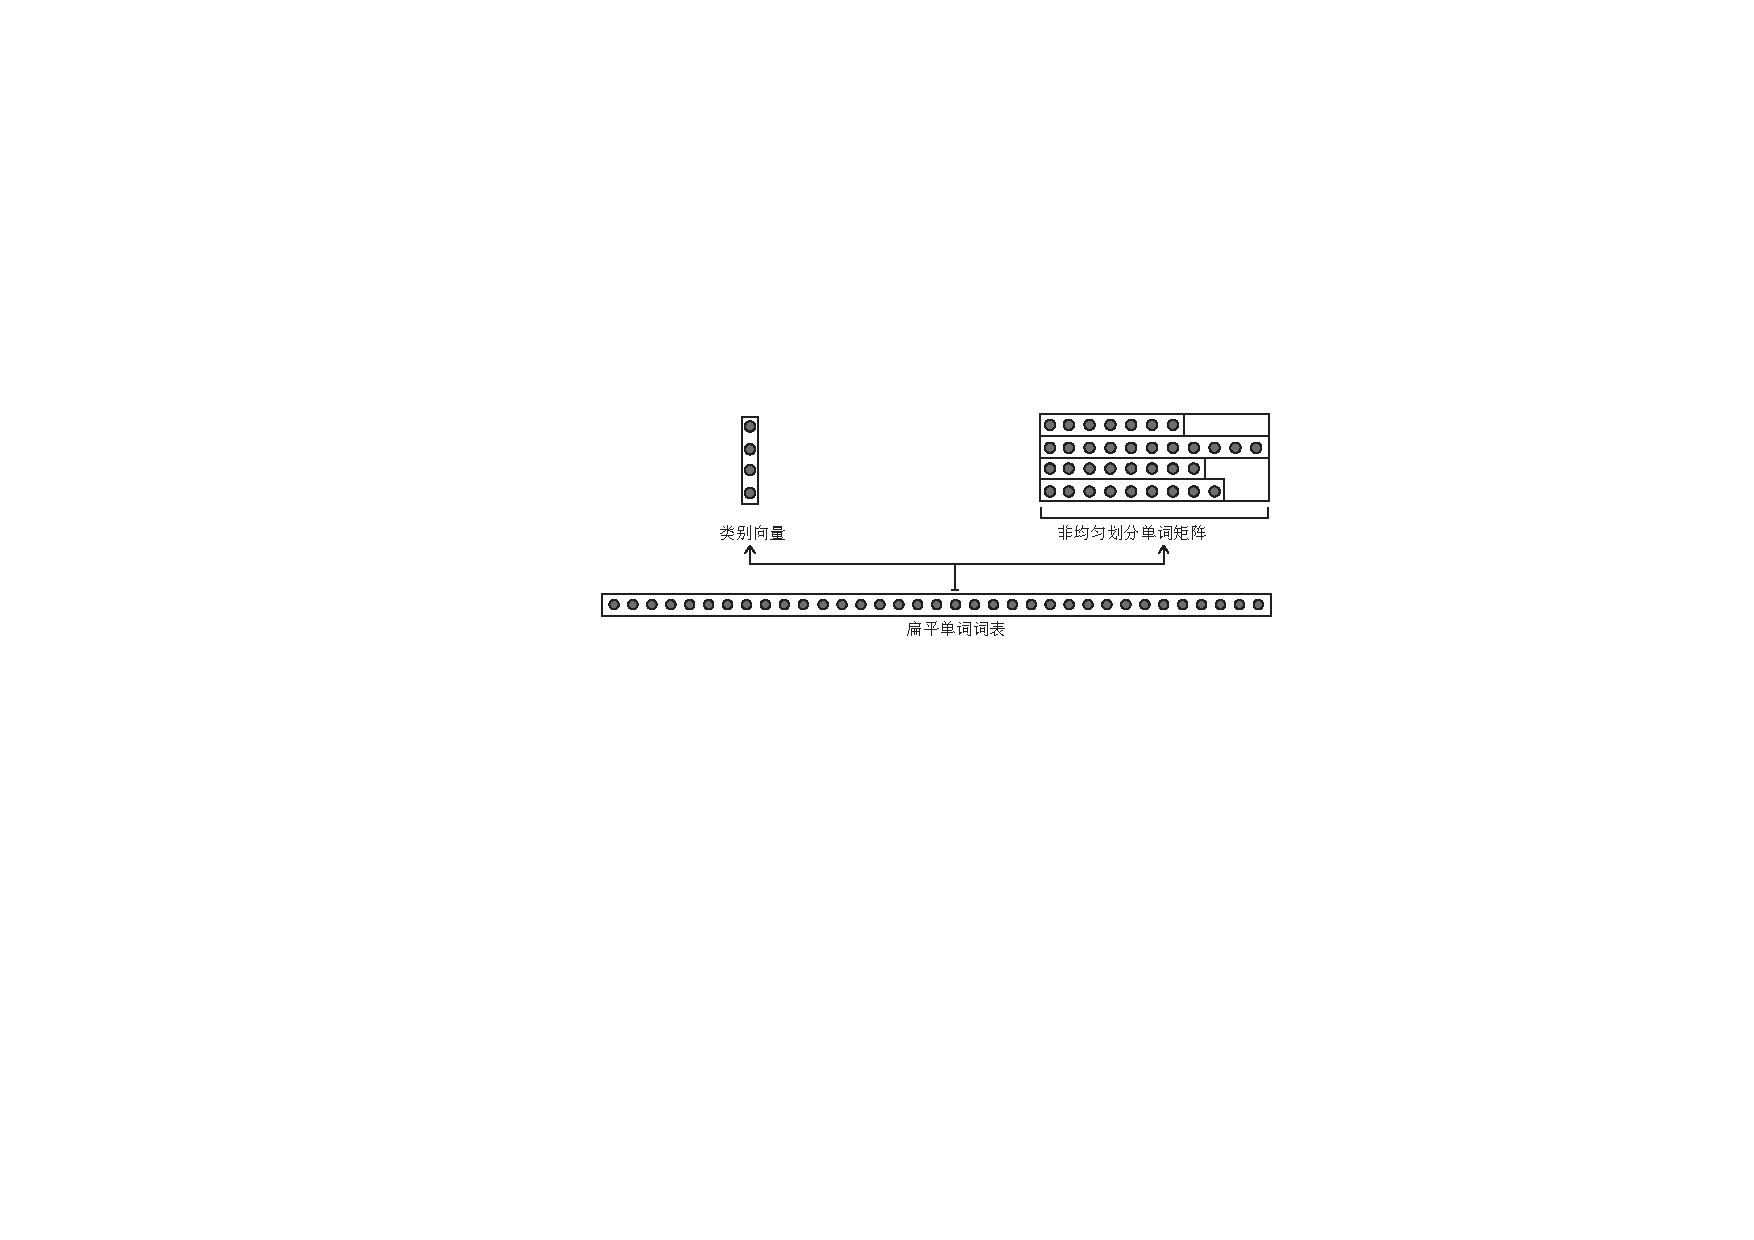
\includegraphics[width=0.85\linewidth]{./figures/chsm-simple.pdf}
\caption{cHSM算法的两种不同的词表划分算法}\label{fig:chsm}
\end{figure}


更重要的是,我们将一次性索引设置分成一个元组$(w ^ c,w ^ o)$,可以从查找表$\Gamma $中检索给定单词索引$ w $。此外,$ w ^ c $指定类ID,$ w^c $表示该组内的本地单词索引。
\begin{equation}\label{equ:partition}
 \theta^m=
\begin{cases}
    \text{单位矩阵} ,& \text{若均匀划分} \\
    \text{掩码矩阵},   & \text{否则}
\end{cases}
\end{equation}


如图~\ref{fig:chsm}~所示,扁平化的词汇可以形成右上矩阵,矩阵的大小应该大于或等于词汇表,不需要外部掩码。
另外,拼合词汇可以形成左上矩阵,需要外部掩模,矩阵的构成依赖于分割算法。

\section{基于类别的代价函数和导数}
给定最后一个隐藏层输出$ h $,那么这个分区组中的每个组和每个单词的概率可以被定义为:
\begin{equation}
\begin{split}
\log p^c(c|h) &= \theta^c h-\log \sum{\exp( \theta^c h )} \\
\log p^g(w|w^c,h)&=\theta^o h -\log\sum\exp{(\theta^o h)}
\end{split}
\end{equation}
其中$ p ^ c $和$ p ^ w $是分别计算而不是并行计算的,因为主要的计算瓶颈是局部标准化的单词概率$ p ^ w $,所以这两个概率的并行计算不会达到时间效率提升。


尽管如此,掩码矩阵不能直接应用于这个分词矩阵,应该应用在log softmax概率计算程序中。 为了说明,在softmax函数中:$ p(x_i)= {\exp({x_i}})/ {\sum_j \exp(x_j)} $,如果$ x_k = 0 $,但其概率$ p(x_k)> 0,\quad \exp(x_k)> 0 $。 因此,该组中确切的后验词对数概率计算如下:
\begin{equation}
  \log p^o(w|w^c,h)=\theta^o h -\log\sum\theta^m\exp(\theta^o h)
\end{equation}

那么,这个模型的损失函数可以形式化如下:
\begin{equation}
\ell(\theta|h) =\log p^c(w^c|h) +\log p^o(w^o|w^c,h)
\end{equation}
其中类别水平损失等于负对数似然的常见设置,并且字水平损失需要在计算其损失时指定其类别 $ w ^ c $。

在训练过程中,$ w ^ c $是预定义的,在测试过程中,$ w ^ c $由$ \arg\max_c p ^ c $获取。 类似地,关于梯度,模型的参数被优化。
\begin{equation}
\begin{split}
\frac{\partial \ell}{\partial \theta^c}=& (\delta_{ij}-p(c|h))h \\
\frac{\partial \ell}{\partial \theta^o}=&(\delta_{ij}-p(w|c,h))h \\
\frac{\partial \ell}{\partial h}=&(\delta_{ij}-p^c(c|h))\theta^c + (\delta_{ij}-p^o(w|c,h))\theta^o
\end{split}
\end{equation}

将词汇分成相互排斥的词组的一个主要优点是:a)避免了在整个词汇表上规范概率。 由于$ p ^ c $是在类维度上标准化的,$ p ^ o $是在最大组大小上进行标准化的。 所以在第二个方程中,多余的其他组被忽略,在最大的文本数据集中二者都不会超过1000。 b)与基于树的结构相比,它在词汇表上的分布更少,在分解步骤中丢失的信息更少。 c)与子字级方法相比,它不会增加序列长度,也不会影响复发性细胞的长程依赖性建模。



\section{基于类别的测试推理}
在推理阶段,对于cHSM模型来说,序列的概率评分要容易得多。
类似于以前的方法,我们可以通过重新研究我们的训练模型来解决第一个问题:
\begin{equation}\label{equ:class_inf}
   \log p(w_1,\cdots, w_T)=\sum_t^T\log p(w_t|h_t)=\sum_{t=1}^{T}\log p^c(w^c_t|h_t) +\log p^o(w^o_t|w^c_t,h_t)
\end{equation}
我们发现这种类型的操作比传统的softmax方法有效得多,该方法涉及$ \mathcal{O (| H | \sqrt{|V|} )}$计算。

其次,对于$\arg\max $的情况,我们可以在选择最佳候选项之前计算词汇表中所有单词的概率,这在直观上是正确的,但在
,因为涉及到整个单词的分割矩阵。 此外,我们仍然可以在算法~\ref{alog:exact}~中对上述方法进行少量修改,然后计算确切的最高候选人。
\begin{algorithm}[!ht]
\caption{基于 cHSM 算法的正确 $\arg\max$ 算法}\label{alog:exact}
\KwData{ 隐藏层输出 $h$;}
\KwResult{ The predicted best candidate word $w$.}
 $\hat y^o=\arg\max_o{\log p^o(w| c,h)}$ \tcp*[r]{select best candidates in every group}
 $\tilde y^c=\arg\max_c{(\log p^c(y^c|h)+\log p^w(\hat y^w|\hat y^c,h))}$\tcp*[r]{calculate best candidate}
 alter $(\tilde y^c,\hat y^o[\tilde y^c])$ with word $w$ by looking-up table $\Gamma'$ \;
 \Return $w$ \;
\end{algorithm}

此外,cHSM算法的性能对词表划分算法有些敏感,因为某些方法可能会产生高度不平衡的字组,并且这种偏斜的分布会在算法中产生标签偏差问题。第一个本地 $\arg\max_o$ 进程~\upcite{DBLP:conf/icml/LaffertyMP01}。然而,在大多数情况下,如果选择合适的参数,则可以考虑不平衡的问题,本文考虑平衡词汇分区的广义形式。

为了说明,考虑两个类 $ c_p $ 和 $ c_q $,这两个类的容量是不同的,例如 $| c_p | \le | c_q |$。在计算了最后一个隐藏层输出 $h$与类图层参数的相似性之后,我们继续计算 $h$ 与每个组的内部单词 $w$ 的相似性得分,这些单词在每个特定组中都没有进行局部规范化整个词汇。当$ | c_p | \approx|c_q|$ 表示我们希望将词汇聚类成等大小的群组,而不是高度倾斜的群组分布时,可以减轻标签偏差问题,其中$ | c_p | \ll | c_q | $ 。更具体地说,对于分布不均的情况,对于类 $ c_q $中的单词来说这个概率被一大群单词稀释是不公平的,这样算法更有可能以较高的概率取出这个小组中的单词,放弃在其他大集团有更多的潜在的话。

我们可以用局部贪婪算法搜索次优结果,而不是搜索确切的全局最优结果,而是建议将这个$ \arg\max $进程分解为两个阶段:a)计算类概率,并剔除顶端一个$ \hat c $; b)计算该类别的单词概率$ \hat c $,并选择具有最高本地单词概率的单词。这个算法会给psudo最好的候选人,但是与原始算法~\ref{alog:exact}相比,它的运行速度要快得多。而且,由于分组词在本地进行归一化,标签偏差问题可以在一定程度上缓解。在实验研究中将讨论算法~\ref{alog:exact}和~\ref{alog:argmax}的详细不同性能。
\begin{algorithm}[!ht]
\KwData{隐藏层输出 $h$;}
\KwResult{ 最佳的候选单词 $\hat w$.}
 $\hat w^c=\arg\max_c{\log p^c(c|h)}$ \tcp*[r]{select best candidate among classes}
 $\hat w^o=\arg\max_o{\log p^o(w|\hat w^c,h)}$\tcp*[r]{select best candidate in specific group}
 alter $(\hat w^c,\hat w^o)$ with word $\hat w$ by looking-up table $\Gamma'$ \;
 \Return $\hat w$
 \caption{基于 cHSM 模型伪 $\arg\max$ 算法}\label{alog:argmax}
\end{algorithm}

\subsection{词表划分算法}
由于cHSM模型的性能与其词汇分割算法密切相关,我们将聚类算法的现有工作进行汇总,并将可能的方法分类如下:

1)随机初始化。 这种直观的方法忽略了单词的所有外部信息,因此单词与随机随机播放过程是等分的。这是揭示其他聚类方法下界的最坏情况,也可以揭示应用高级聚类策略的相对收益。

2)字母顺序。 这种方法根据字符级别的信息对单词进行排序,同一组中的单词共享一个相似的子字符串。

3)Unigram 聚类。这些单词首先根据它们在文本中的频率排序,然后通过放置边界使得每个类别占总概率质量的恒定部分,从而形成连续单词块。这种方法具有这样的性质:较低编号的类比较高编号的类具有更少的成员,因为它们的成员更频繁~\upcite{DBLP:conf/nips/MikolovSCCD13}。

4)Bigram聚类。它是指布朗聚类方法,这是历史适用于基于n-gram的基于类的模型~\upcite{DBLP:journals/coling/BrownPdLM92,liang2005semi}。单词使用相同的bigram上下文分组到相同的行中。

5)结构聚类\footnote{https://github.com/AlonDaks/unsupervised-authorial-clustering}。根据文本中的单词的词性和句法结构划分词表~\upcite{daks2016unsupervised} 。

4)语义聚类。我们将传统的kmeans聚类方法应用到预训练的词嵌入,使得我们可以通过指定聚类的大小将词汇分成不同的形状。
\section{本章小结}